\subsection{MVP}
\label{MVP}
MVP (Model-View-Presenter) ist ein Design Pattern. Es ist ähnlich dem MVC
(Model-View-Controller). Google beschreibt den Nutzen des MVP Patterns in der
Einbindung von Testfällen in einer GWT Anwendung. Darüber hinaus kann dieses
Pattern auch genutzt werden um eine GWT Anwendung für verschiedene Plattformen
verfügbar zu machen z.B. für Browser auf mobilen Endgeräten oder auf dem
Desktop.
\begin{figure}[htbp]
\begin{center}
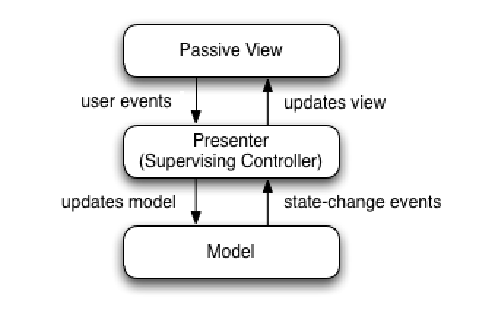
\includegraphics{./img/MVP.pdf}
\caption{Visualisierung des MVP Patterns \cite{bib:MVP1}}\label{Fig:MVP}
\end{center}
\end{figure}\\
Bei MVP übernimmt der Presenter die Logik und die View ist einfach gehalten
\cite{bib:MVP2}. Dies sorgt für eine klare Trennung zwischen Model und View (vgl.
Abbildung \ref{Fig:MVP}). Wohingegen bei MVC die View das Model kennt
\cite{bib:MVCvsMVP}. Der Presenter steuert die View und übermittelt die Daten
des Models zur View.
Dadurch wird der einfache Austausch von Views ermöglicht ohne das weitere
Änderungen vorgenommen werden müssen \cite{bib:MVP1}\cite{bib:MVP2}.

In der zu generierenden Anwendung soll das MVP Pattern ohne ein konkretes Model
implementiert werden, da ausschließlich eine GWT Frontend Anwendung generiert
werden soll. Die MVP Struktur ist dabei so umgesetzt, sodass der Presenter als
Interface in dem View Interface enthalten ist und über eine Activity definiert
wird, welche zusätzlich für das Event handling und die Datenbeschaffung verantwortlich
ist. Die konkrete Implementierung der View beinhaltet das Presenterobjekt, damit
dadurch die Aktionen der View Komponenten (bei GWT Widgets) an den Presenter
übergeben werden können.
